We then explore the impact of receive antenna $U$ and subband $N$ on the R-E region for MIMO systems with transmit antenna $M = 2$ over a typical FF channel. The dominant eigenvalue of each subband is shown in Fig. \ref{fig:mimo-channels}.

\begin{figure}[ht]
  \centering
  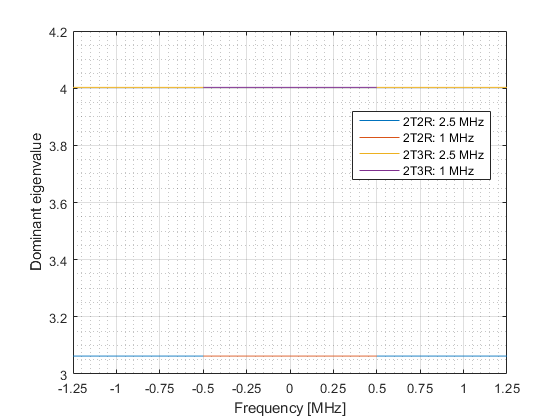
\includegraphics[width=0.5\textwidth]{mimo_frequency_flat_mimo_channel}
  \caption{Frequency response of the MIMO FF channel}\label{fig:mimo-channels}
\end{figure}

\begin{figure}[ht]
  \centering
  \subfigure[FF: $N = 2$]{
    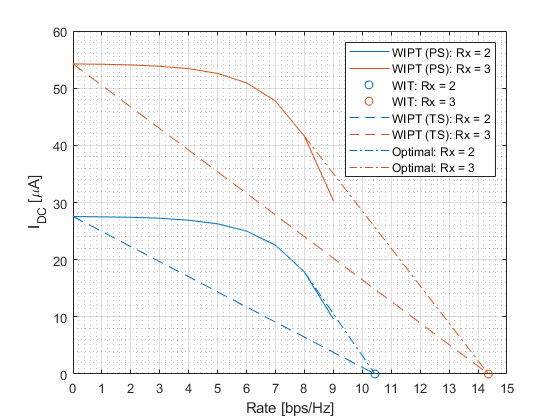
\includegraphics[width=0.48\textwidth]{mimo_re_subband_2}\label{fig:mimo-re-subband-2}}
  \subfigure[FF: $N = 4$]{
    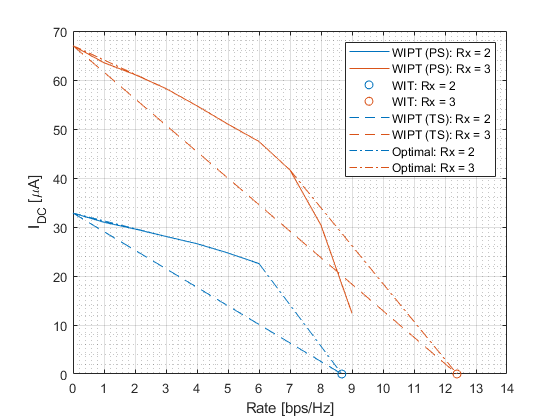
\includegraphics[width=0.48\textwidth]{mimo_re_subband_4}\label{fig:mimo-re-subband-4}}
  \caption{R-E region vs $N$ and $U$ for MIMO FF channels}
  \label{fig:re-mimo}
\end{figure}

As illustrated in Fig. \ref{fig:re-mimo}, a contrast between $U = 2$ and 3 suggests that increasing $U$ may boost the rate and energy simultaneously, thanks to the multiplexing gain of MIMO. For a fixed $M = 2$, increasing $U$ from 2 to 3 provides no extra streams for transmission but produces a larger channel eigenvalue, which benefits the R-E region by increasing the effective subband amplitude.

On the other hand, a large $N$ amplifies the harvested power as expected from the rectifier nonlinearity. It can be observed that the R-E curves begin to show some concavity-convexity for $N = 4$, which was first observed for $N = 8$ in SISO channels. A possible reason is that each subchannel in this case has 2 virtual streams so that the equivalent subband is indeed $4 \times 2 = 8$. Therefore, MIMO demonstrates a twofold benefit in rate and energy. It requires a smaller $N$ to achieve a certain output power level and is more suitable for PAPR-constrained devices.

The main problem of the plot is that the rightmost points of the R-E curves do not reach the x-axis. It results from the discrete rate constraints employed in the simulation. With a step of 1 bps/Hz, the points tend to locate near the integer rates. For instance, the plot corresponding to $U = 2$ and $N = 4$ terminates at a rate of 6 bps/Hz with an output current of \SI{22}{\uA}, indicating the proposed PS-WIPT strategy cannot achieve the next rate milestone of 7 bps/Hz. The reason is that the suboptimal phases ${{\mathbf{\Phi }}_P^\prime ,{\mathbf{\Phi }}_I^\prime }$ are determined before the optimization so that the algorithm cannot reach the channel capacity corresponding to WIT. Therefore, the proposed GP approach is suboptimal for MIMO systems.

For a fixed $M$ and $U$, a good R-E tradeoff can be obtained by a combination of the following strategies. In the low-rate region, we can use PS-WIPT for a small $N$ and employ TS between WPT and WIPT for a large $N$. In the medium-rate region, PS-WIPT can generally guarantee a decent tradeoff between rate and energy. When the rate constraint is high, TS between WIT and WIPT is the best strategy to enjoy the benefit of multisine and avoid the rate loss of suboptimal phases.

Despite as expected, the conclusions require more evidence since only one specific channel is investigated in the simulation. 